\documentclass[conference]{IEEEtran}

\usepackage[utf8]{inputenc}
\usepackage[T1]{fontenc}
\usepackage{graphicx}
\usepackage{amsmath}
\usepackage{booktabs}
\usepackage[hyphens]{url}
\usepackage{multirow}
\usepackage{microtype}

\IEEEoverridecommandlockouts

\begin{document}

\title{Where Does Autoscaling Latency Come From?\\
A Measurement Study of the Kubernetes Horizontal Pod Autoscaler}

\author{\IEEEauthorblockN{Ricardo Kenzo Akaki Ito}
\IEEEauthorblockA{\textit{Escola Polit\'ecnica} \\
\textit{Universidade de S\~ao Paulo}\\
S\~ao Paulo, Brazil}
}

\maketitle

\begin{abstract}
The Kubernetes Horizontal Pod Autoscaler (HPA) is commonly characterized by its
reconciliation period, and practitioner guidance concentrates on tuning
autoscaler policies. This paper reports a measurement study showing that, in a
default single-node deployment, the autoscaler accounts for only a small
fraction of the observed reaction time. Using an open-loop load generator
calibrated in offered CPU cores and a ground-truth temporal reference, we
decompose the interval between load onset and the creation of the first
additional replica into a metrics-pipeline component and a controller
component. Across twelve phase-randomized runs, the metrics pipeline accounted
for 49.4~s on average while the controller accounted for 5.8~s. The delay is
not a constant but a random variable whose spread matches one metrics
collection cycle, ranging from 28~s to 77~s with a 49~s amplitude against a
60~s declared resolution. Varying the collector resolution from 15~s to 60~s
changed the time to reach the replica ceiling by a factor of 3.7, an effect
larger than that of any autoscaler parameter we swept. We further show that a
previously reported detection latency of 16~s, obtained by the authors in an
earlier study, was a measurement artifact produced by reading two fields of the
same stale controller status. These results suggest that responsiveness work
should target the observability path before autoscaler policy.
\end{abstract}

\begin{IEEEkeywords}
Kubernetes, horizontal pod autoscaling, elasticity, performance measurement,
cloud computing
\end{IEEEkeywords}

\section{Introduction}

Elasticity is frequently presented as the defining property of cloud computing.
In container orchestration platforms, this property is realized by concrete
mechanisms, and the Horizontal Pod Autoscaler (HPA) is the most direct among
them. The HPA follows the reconciliation model that characterizes Kubernetes.
An operator declares a desired state, expressed as a replica range and a
utilization target, and a controller continuously compares that declaration
against the observed state, acting when they diverge.

At each control cycle, whose default period is fifteen seconds, the controller
queries a utilization metric and computes the required number of replicas as
\begin{equation}
r_{\text{desired}} = \left\lceil r_{\text{current}} \times
\frac{u_{\text{current}}}{u_{\text{target}}} \right\rceil
\end{equation}
where $u$ denotes the mean utilization of the replicas, measured as a fraction
of the CPU declared in the container's resource requests.

Because this control period is the most visible parameter of the mechanism, the
reaction time of the HPA is often characterized by it, and practitioner guidance
concentrates on tuning autoscaler policies such as utilization targets,
stabilization windows and scaling rates. The utilization metric itself, however,
does not originate in the controller. It is produced by a separate component,
the Metrics Server, which scrapes the kubelet at its own independent period and
computes CPU usage from cumulative counters, therefore requiring two consecutive
samples before any value can be reported.

This paper asks a question that follows directly from that separation. When a
workload experiences a sudden load increase, how much of the delay until
additional replicas appear is attributable to the autoscaler, and how much to
the path that makes the metric visible to it?

The question is practically motivated. If the controller dominates, tuning HPA
policies is the appropriate intervention. If the observability path dominates,
policy tuning optimizes the smaller term and responsiveness work should be
directed elsewhere.

\subsection{Relation to prior work by the author}

This study extends an earlier comparative experiment conducted by the author,
in which the same application was deployed to a local Minikube cluster and to a
managed Amazon EKS cluster and subjected to load~\cite{prev}. That study
reported a detection latency of approximately 16~s in both environments and
concluded that the latency was governed by the controller's reconciliation
period and was therefore independent of the underlying infrastructure.

One contribution of the present work is to show that this conclusion does not
hold, and that it followed from a defect in the instrumentation rather than from
the behavior of the system. Section~\ref{sec:artifact} documents the defect, its
effect on the reported values, and the corrected measurement procedure.

\subsection{Contributions}

\begin{itemize}
\item A measurement methodology that establishes a ground-truth temporal
reference for load onset, avoiding inference from controller-reported metrics
that are themselves delayed.
\item An open-loop load generator calibrated in offered CPU cores rather than
in client concurrency, making offered load comparable across environments with
different processing capacity, and reporting the load it actually sustained.
\item A decomposition of autoscaling reaction time into a metrics-pipeline
component and a controller component, measured rather than assumed.
\item Evidence that detection delay is a random variable whose dispersion
matches one metrics collection cycle, and that reporting it as a single value
is therefore insufficient.
\item Identification and correction of a measurement artifact in previously
reported results.
\end{itemize}

\section{Background and Related Work}

\subsection{The autoscaling path}

Three components participate in a CPU-driven scaling decision. The kubelet on
each node exposes cumulative CPU counters for running containers. The Metrics
Server periodically scrapes these counters and derives a usage rate, which
requires at least two samples separated by the collection interval. The HPA
controller queries the resulting metric at its own period and applies~(1).

Each component contributes latency, and the contributions are additive but not
equal. The controller period bounds how often a decision can be made. The
collection interval bounds how recent the information behind that decision can
be. Since usage is derived from differences between cumulative counters, the
metric describing an interval only becomes available after the interval closes,
which introduces a delay of at least one collection period even under ideal
alignment.

\subsection{Reported characterizations}

Documentation and practitioner material commonly describe HPA responsiveness in
terms of the controller period and of policy parameters under operator control.
The Kubernetes documentation describes the reconciliation period and the
behavior policies that govern scaling rate and stabilization~\cite{k8shpa}. The
Metrics Server project documents its resolution parameter and recommends values
compatible with the autoscaler, but the interaction between the two periods is
rarely quantified in applied reports.

The distinction matters because the two parameters are configured by different
actors. The HPA period and policies are set per workload, in manifests that
application teams own. The collector resolution is a property of a
cluster-scoped component, frequently installed by a distribution or platform
team with defaults that application teams neither choose nor observe.

\subsection{Scope}

This study addresses a single-node cluster with CPU-based scaling and does not
consider node autoscaling, custom metrics, or vertical scaling. The restriction
is deliberate. Introducing node provisioning would add an independent and
substantially larger latency term, which would obscure the comparison between
the two components examined here.

\section{Methodology}

\subsection{Workload}

The workload is a small HTTP server written in Python with no external
dependencies. It exposes a health endpoint that responds immediately and is used
as the target of readiness and liveness probes, and a work endpoint that
consumes processor time deliberately.

The work endpoint consumes CPU for a \emph{target duration} rather than for a
fixed number of iterations. This is a methodological requirement rather than an
implementation convenience. Under an iteration-based definition, a faster
processor completes the work sooner and consumes fewer CPU-seconds per request,
so part of any difference observed between environments would originate in
hardware rather than in the mechanism under study. Fixing the CPU time makes
each request cost approximately the same CPU-seconds everywhere.

Measured accuracy is adequate for this purpose. For a 200~ms target, the
observed consumption was 200.34~ms, an error of 0.17\%.

The application is packaged from \texttt{python:3.12-slim}, runs as an
unprivileged user, and is published under an immutable tag so that every
execution is guaranteed to run identical code.

\subsection{Load generation}

Load is applied by a generator executing inside the cluster. An external
generator would traverse a network path absent in the local case and would
require exposing the service through a load balancer, neither of which is
desirable for a controlled comparison.

The generator operates in \emph{open loop}. Request dispatch instants are
scheduled at fixed intervals derived from the target rate, computed from the
start of the run rather than accumulated from the previous dispatch, so that
transient delays do not permanently shift the time base. This contrasts with the
closed-loop generator used in the prior study, which issued the next request
only after the previous response arrived, making the effective rate a function
of server latency and client capacity.

Because the work endpoint consumes a known amount of CPU per request, offered
load is expressed in cores:
\begin{equation}
\text{offered cores} = \text{rate} \times \text{cost per request}
\end{equation}
With a cost of 50~ms, a rate of 40~requests per second corresponds to
2.0~offered cores. The specification therefore carries the same physical meaning
in any environment.

The generator also measures what it achieved. It reports the rate observed in
each reporting window, not only the cumulative rate. This distinction is
necessary because the experiment begins with a single replica that cannot serve
the offered rate, so the cumulative figure is depressed for physical reasons
during the ramp. Load validity is assessed on windows after scaling completes;
observed adherence in steady state was between 0.985 and 1.005 across runs.

\subsection{Temporal reference}
\label{sec:artifact}

The prior study inferred the instant of load onset from the first sample in
which the utilization reported by the HPA exceeded the configured target. That
inference is unsound, because the reported utilization is refreshed only once
per controller cycle and is itself derived from a delayed collection.

The defect had a second and more damaging consequence. Replica counts were read
from \texttt{status.currentReplicas} of the HPA object, which is refreshed on
the same cycle, whereas readiness counts were read from the Deployment, which is
updated continuously. Samples were therefore internally inconsistent: we observed
records reporting five ready replicas while the same record reported one
existing replica, which is impossible.

Since both the reference instant and the replica count were drawn from the same
delayed source, the interval between them measured the controller cycle against
itself. This explains the previously reported value of approximately 16~s and
its apparent stability across environments.

The corrected instrumentation makes three changes. Replica counts are read from
the Deployment and independently verified by direct enumeration of pods.
Controller-reported counts are retained in a separate column, so that the lag
between decision and observed state remains visible rather than conflated.
Finally, the orchestrator records the wall-clock instants at which load was
applied and removed, and the analysis uses these markers as the temporal
reference.

\subsection{Experimental design}

All runs share a fixed procedure. The deployment is reset to a single replica,
the autoscaler is applied with the parameters of the experimental point, the
collection begins, a baseline interval is recorded at rest, load is applied,
and observation continues through the reduction phase. Each run is executed
without supervision to eliminate procedural variation between repetitions.

Four sweeps isolate one factor each, holding the others at reference values of
40~requests per second, a 50\% utilization target and a 300~s stabilization
window:

\begin{itemize}
\item \textbf{A}, utilization target at 30\%, 50\% and 70\%;
\item \textbf{B}, offered load at 1.0, 2.0 and 4.0 cores;
\item \textbf{C}, downscale stabilization window at 60~s, 180~s and 300~s;
\item \textbf{D}, metrics collector resolution at 15~s, 30~s and 60~s.
\end{itemize}

A fifth experiment, described in Section~\ref{sec:phase}, repeats a single point
twelve times with a randomized delay before load application.

\subsection{Environment}

Experiments ran on a single-node Minikube cluster with four virtual CPUs and
4~GiB of memory, hosted on a notebook running Ubuntu Server 24.04, Kubernetes
v1.35.1, Metrics Server v0.8.1. The distribution's default collector resolution
is 60~s, a value we discovered during this study and which is central to the
results reported below. Each replica requests 100~millicores, and the autoscaler
range is one to ten replicas.

\section{Results}

\subsection{Detection delay is not a constant}
\label{sec:phase}

Sweeps over autoscaler parameters produced differences between cells that admit
no physical explanation. Under sweep~B, the intermediate load level exhibited a
detection delay three times larger than both extremes, with a standard deviation
of 23.6~s against approximately 3~s at neighboring points. A larger offered load
being detected later than a smaller one is not a plausible mechanism.

We hypothesized \emph{phase alignment} with the collection cycle. Since the
collector samples at fixed intervals, the delay before a load change becomes
visible depends on where the onset falls within that interval. Load starting
just before a scrape becomes visible almost immediately; load starting just
after waits nearly two intervals. Because each experimental point has a fixed
duration, its repetitions tend to fall at the same phase, which produces
artificially low variance within cells and apparent differences between them.

To test this, a single point was repeated twelve times with a delay drawn
uniformly from $[0, 60)$~s inserted before load application, randomizing phase.

\begin{table}[ht]
\caption{Detection delay under randomized phase ($n=12$)}
\label{tab:fase}
\centering
\begin{tabular}{@{}lr@{}}
\toprule
Statistic & Value \\
\midrule
Minimum          & 28.0~s \\
Maximum          & 77.0~s \\
Mean             & 55.2~s \\
Median           & 53.5~s \\
Standard deviation & 17.2~s \\
Amplitude        & 49.0~s \\
\midrule
Declared collector resolution & 60~s \\
\bottomrule
\end{tabular}
\end{table}

\begin{figure}[t]
\centering
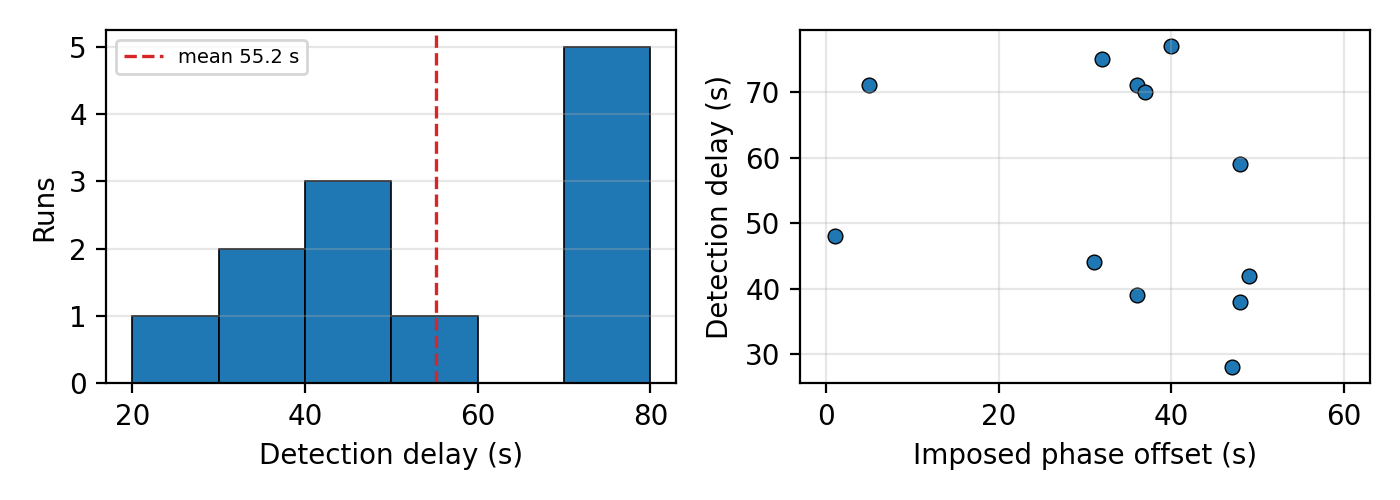
\includegraphics[width=\columnwidth]{figuras/atraso_distribuicao.png}
\caption{Detection delay under randomized collection phase. Left, distribution
over twelve runs with all configured parameters held fixed. Right, delay against
the imposed phase offset. The spread of 49~s is comparable to one 60~s
collection cycle.}
\label{fig:dist}
\end{figure}

Table~\ref{tab:fase} and Fig.~\ref{fig:dist} report the resulting distribution. The observed amplitude
of 49~s is consistent with one collection cycle, supporting the hypothesis. The
delay ranges over a factor of 2.75 between its smallest and largest observed
values while every configured parameter remains fixed.

The practical implication is that a single reported value does not characterize
this quantity. For capacity planning, the relevant figure is the upper bound
rather than the mean, since it determines worst-case exposure to unserved load.

\subsection{Decomposition of the reaction time}

The same twelve runs allow the delay to be separated into its two components.
The first extends from load application until the utilization reported to the
controller exceeds the target. The second extends from that instant until the
first additional replica exists.

\begin{table}[ht]
\caption{Decomposition of detection delay ($n=12$)}
\label{tab:decomp}
\centering
\begin{tabular}{@{}lrr@{}}
\toprule
Component & Mean & Share \\
\midrule
Load onset to metric visibility & 49.4~s & 89.5\% \\
Metric visibility to first replica & 5.8~s & 10.5\% \\
\midrule
Total & 55.2~s & 100\% \\
\bottomrule
\end{tabular}
\end{table}

\begin{figure}[t]
\centering
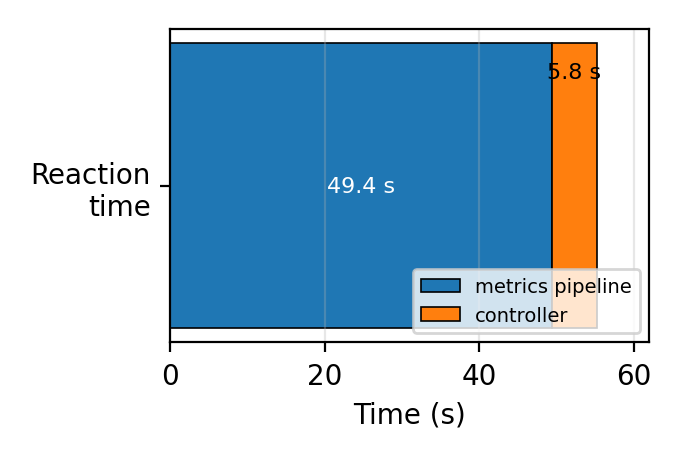
\includegraphics[width=0.78\columnwidth]{figuras/decomposicao.png}
\caption{Mean decomposition of the interval between load onset and the first
additional replica. The controller accounts for 5.8~s of a 55.2~s total.}
\label{fig:decomp}
\end{figure}

Table~\ref{tab:decomp} and Fig.~\ref{fig:decomp} present the result. The controller required less than
six seconds on average to observe the metric, decide, and produce additional
replicas. Approximately 90\% of the reaction time elapsed before the controller
had any information to act upon.

In eight of the twelve runs the two instants coincided within the five-second
sampling interval, indicating that the controller acted on the first sample in
which the metric crossed the target.

This is the central result of the paper. The component that practitioner
guidance targets is responsible for roughly one tenth of the latency observed.

\subsection{Collector resolution dominates}

Sweep~D varied the collector resolution while holding all autoscaler parameters
fixed.

\begin{table}[ht]
\caption{Effect of collector resolution (sweep D, $n=3$ per cell)}
\label{tab:res}
\centering
\begin{tabular}{@{}lrrr@{}}
\toprule
 & 15~s & 30~s & 60~s \\
\midrule
To first replica (s) & $21.3 \pm 5.8$ & $44.0$ & $45.7 \pm 2.9$ \\
To ceiling (s)       & $44.3 \pm 0.6$ & $60.0$ & $164.0 \pm 3.5$ \\
Replicas at peak     & 10 & 10 & 10 \\
\bottomrule
\end{tabular}
\end{table}

\begin{figure}[t]
\centering
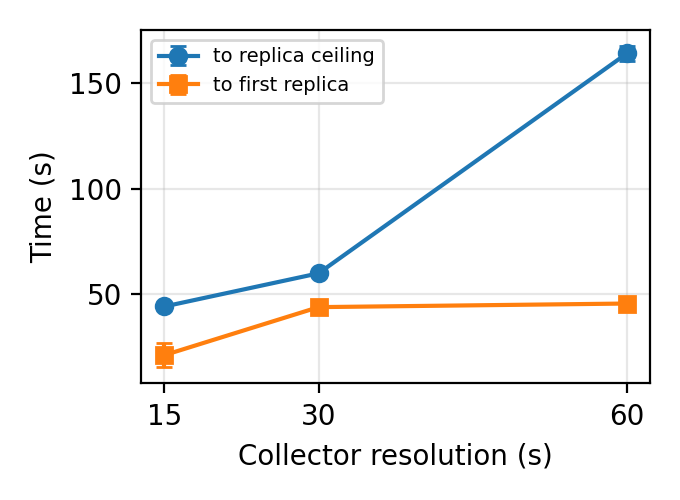
\includegraphics[width=0.78\columnwidth]{figuras/resolucao.png}
\caption{Effect of metrics collector resolution on scaling time, with all
autoscaler parameters held fixed. Time to the replica ceiling grows by a factor
of 3.7 between 15~s and 60~s resolution.}
\label{fig:res}
\end{figure}

Table~\ref{tab:res} and Fig.~\ref{fig:res} show the time to reach the
ten-replica ceiling growing from
44~s to 164~s, a factor of 3.7, as resolution coarsens from 15~s to 60~s. No
autoscaler parameter examined in this study produced an effect of comparable
magnitude.

The shape of the response is informative. Time to the \emph{first} replica
saturates between 30~s and 60~s, whereas time to the \emph{ceiling} continues to
grow. Each successive scaling step requires a fresh metric, so the collection
penalty is incurred once per step and accumulates along the scaling sequence
rather than only at its start.

\subsection{Cost of finer collection}

Recommending a shorter collection interval is incomplete without accounting for
its cost. Collection consumes resources in the Metrics Server and imposes
requests on each kubelet, and the latter scales with cluster size.

We measured the Metrics Server's own consumption at each of the three
resolutions, sampling five times per configuration after allowing the component
to stabilize.

\begin{table}[ht]
\caption{Metrics Server consumption by collection resolution}
\label{tab:custo}
\centering
\begin{tabular}{@{}lrr@{}}
\toprule
Resolution & CPU & Memory \\
\midrule
60~s & 4~m & 21~MiB \\
30~s & 3--4~m & 18~MiB \\
15~s & 3--4~m & 18~MiB \\
\bottomrule
\end{tabular}
\end{table}

No difference is discernible in Table~\ref{tab:custo}. Three caveats bound what
this permits us to conclude.

First, the reporting granularity is one millicore, so the variation between
3~m and 4~m is a rounding step rather than a measurement. A fourfold increase
in a quantity below one millicore would be invisible at this scale. The
appropriate statement is that the difference falls below the resolution of the
instrument, not that it is zero.

Second, the cluster has a single node. Collection cost grows with node count,
since the component scrapes each kubelet every interval. A result obtained on
one node does not transfer to a cluster of hundreds.

Third, the Metrics Server was measured by the Metrics Server, whose averaging
window is the very parameter under variation. At 60~s resolution the reported
value averages over 60~s, and at 15~s over 15~s, so the figures are not strictly
comparable to one another.

Within these limits, the measurement supports a narrow claim. At single-node
scale, moving from 60~s to 15~s collection produced no cost increase detectable
by the cluster's own instrumentation, while reducing time to the replica ceiling
from 164~s to 44~s. Operators of larger clusters should measure the cost in
their own environment before adopting the change.

\subsection{Autoscaler parameter sweeps}

Sweeps A, B and C are reported as a negative result. Their between-cell
differences are not separable from phase effects at the sample sizes used.

\begin{table}[ht]
\caption{Autoscaler parameter sweeps ($n=3$ per cell)}
\label{tab:abc}
\centering
\small
\begin{tabular}{@{}llrr@{}}
\toprule
Sweep & Level & To first replica (s) & To ceiling (s) \\
\midrule
\multirow{1}{*}{A} & target 30\% & $28.3 \pm 0.6$ & $104.3 \pm 3.2$ \\
 & target 50\% & $51.3 \pm 23.6$ & $136.0 \pm 38.9$ \\
 & target 70\% & $33.7 \pm 31.6$ & $195.0 \pm 3.5$ \\
\midrule
\multirow{1}{*}{B} & 1.0 core & $14.3 \pm 3.2$ & $193.7 \pm 2.9$ \\
 & 2.0 cores & $51.3 \pm 23.6$ & $136.0 \pm 38.9$ \\
 & 4.0 cores & $14.7 \pm 2.9$ & $92.0$ \\
\midrule
\multirow{1}{*}{C} & window 60~s & $45.7 \pm 28.5$ & $114.3 \pm 39.6$ \\
 & window 180~s & $56.0 \pm 16.6$ & $139.3 \pm 46.2$ \\
 & window 300~s & $51.3 \pm 23.6$ & $136.0 \pm 38.9$ \\
\bottomrule
\end{tabular}
\end{table}

Table~\ref{tab:abc} illustrates the difficulty. In sweep~B, detection delay at
1.0 and 4.0 cores is approximately 14~s with small dispersion, while the
intermediate level shows 51.3~s with dispersion an order of magnitude larger.
Since Section~\ref{sec:phase} establishes that this quantity varies from 28~s to
77~s under fixed parameters, cells differing by less than that range cannot be
distinguished at three repetitions.

We report these sweeps rather than omitting them because their failure is
itself informative. Studies that vary autoscaler parameters without controlling
collection phase may attribute to those parameters differences that originate in
the observability path.

One effect does survive. Utilization in steady state tracks offered load
monotonically, at 120\%, 286\% and 387\% for 1.0, 2.0 and 4.0 cores
respectively. This quantity does not depend on the temporal reference and was
not measurable in the prior study, where offered load was not calibrated.

\subsection{Downscale timing}

Sweep~C produced a consistent relation between the configured stabilization
window and the observed onset of reduction: $129.7 \pm 17.0$~s for a 60~s
window, $259.3 \pm 18.5$~s for 180~s, and $375.3 \pm 16.0$~s for 300~s. The
offset is approximately 70~s in all three cases.

Under the previous, defective instrumentation the same measurements yielded
window plus approximately 6~s. The difference is not a new error but the same
correction observed from the opposite direction. Reduction is measured from the
instant load actually ceased, whereas the earlier procedure measured from the
last sample in which the controller still reported high utilization, a quantity
already delayed by the collection path.

The operational consequence is that a configured stabilization window
understates the actual delay before capacity is released, by roughly the
propagation time of the metric.

\section{Discussion}

\subsection{Implications for practice}

The results suggest a reordering of responsiveness work. Before adjusting
utilization targets or scaling policies, operators should establish the
resolution of their metrics collector, since it bounds what any policy can
achieve. A collector configured at 60~s imposes a floor on reaction time that no
autoscaler setting can overcome.

The ordering is supported by the asymmetry between benefit and cost. Moving from
60~s to 15~s reduced time to the replica ceiling by a factor of 3.7 at no cost
detectable by the cluster's own instrumentation, subject to the scale
limitations discussed above. Autoscaler policy tuning, by contrast, operates on
a term that accounted for 5.8~s of a 55.2~s total.

This does not imply that autoscaler parameters are inconsequential. The
stabilization window governed downscale timing precisely and monotonically,
producing 129.7~s, 259.3~s and 375.3~s for configured windows of 60~s, 180~s and
300~s. The claim is narrower: for \emph{detection} latency specifically, the
autoscaler is not the binding constraint.

A second implication follows from the mechanism. Reaching a replica ceiling
requires several successive decisions, each awaiting a fresh metric, so the
collection penalty is paid once per step. Scaling policies that grant larger
increments per step therefore reduce the number of penalties incurred. This is
an autoscaler parameter that does affect responsiveness, though it is not the
one practitioner guidance emphasizes. We did not test it, and it remains open.

This matters because the two parameters are typically owned by different actors.
Application teams configure the HPA in workload manifests they control.
Collector resolution belongs to a cluster-scoped component, often installed with
distribution defaults. In the environment studied, the distribution's default
was 60~s, four times the Metrics Server project's own default, and this was not
apparent from any workload-level configuration.

\subsection{Reinterpreting the prior comparison}

The prior study compared a local cluster against a managed one and found the
managed cluster reached the replica ceiling in 35~s against 74~s locally,
attributing the difference to container runtime and storage. The present results
suggest a simpler explanation. The local cluster used a collector resolution of
60~s, while the managed cluster used the upstream manifest with its 15~s
default. Table~\ref{tab:res} shows that this difference alone accounts for a
factor of 3.7 in time to ceiling.

The earlier conclusion that detection latency was independent of infrastructure
therefore inverted the actual situation. The latency was strongly dependent on
infrastructure, through a component the study did not examine, and the
instrumentation was incapable of revealing this because it measured the
controller cycle against itself.

\subsection{Threats to validity}

\textbf{Single environment.} All measurements come from one single-node cluster.
The decomposition in Table~\ref{tab:decomp} is expected to hold wherever a
collector with coarse resolution is used, but the specific values are not
transferable.

\textbf{Sample size.} Twelve runs characterize the delay distribution and three
runs per cell characterize the sweeps. The latter is insufficient, as
Section~\ref{sec:abc-note} argues, and we report those sweeps with that
limitation stated rather than drawing conclusions from them.

\textbf{Phase coverage.} Randomization drew from a uniform distribution over one
declared cycle. If the effective collection period differs from the declared
resolution, coverage would be incomplete and the reported amplitude would
underestimate the true range.

\textbf{Replica ceiling.} All runs reached the configured maximum of ten
replicas, so the autoscaler operated saturated for part of each run. Measurements
of time to ceiling therefore describe the path to a bound rather than
convergence to the utilization target.

\textbf{Single metric.} Only CPU-based scaling was examined. Custom and external
metrics traverse different pipelines whose latency characteristics may differ.

\label{sec:abc-note}

\section{Conclusion}

This paper measured where autoscaling latency originates in a default Kubernetes
deployment. Under randomized collection phase, the interval between load onset
and the first additional replica averaged 55.2~s, of which 49.4~s elapsed before
the controller had any information to act upon and 5.8~s were attributable to
the controller itself.

The delay is a random variable rather than a constant, with a spread matching
one collection cycle, which implies that single-value characterizations are
inadequate for capacity planning. Varying collector resolution changed time to
the replica ceiling by a factor of 3.7, exceeding the effect of any autoscaler
parameter examined, and did so without a cost increase detectable at
single-node scale.

We also documented a measurement artifact in our own prior work, in which
reading the temporal reference and the replica count from the same delayed
controller status produced an apparent detection latency of 16~s that in fact
measured the reconciliation period against itself.

Three directions follow. Repeating the decomposition on a managed cluster would
test whether the proportion between components holds when the collector is
configured at its upstream default. Extending the analysis to custom metrics
would determine whether pipelines with different architectures exhibit the same
dominance. Finally, combining pod autoscaling with node autoscaling would
introduce a third and larger latency term, whose relative weight has, to our
knowledge, not been characterized alongside the two examined here.

\section*{Availability}

The application source, commented manifests, instrumentation and analysis
scripts, collected time series and execution logs supporting this study are
available in a repository accessible to the course instructors.

\begin{thebibliography}{9}

\bibitem{prev}
R. K. A. Ito, ``Autoescalamento horizontal de Pods em Kubernetes: an\'alise
comparativa entre cluster local e cluster gerenciado,'' course report, PSI5120,
Escola Polit\'ecnica, Universidade de S\~ao Paulo, 2026.

\bibitem{k8shpa}
Kubernetes Documentation, ``Horizontal Pod Autoscaling.'' [Online]. Available:
\url{https://kubernetes.io/docs/tasks/run-application/horizontal-pod-autoscale/}

\bibitem{k8swalk}
Kubernetes Documentation, ``HorizontalPodAutoscaler Walkthrough.'' [Online].
Available:
\url{https://kubernetes.io/docs/tasks/run-application/horizontal-pod-autoscale-walkthrough/}

\bibitem{metrics}
Kubernetes SIGs, ``Kubernetes Metrics Server.'' [Online]. Available:
\url{https://github.com/kubernetes-sigs/metrics-server}

\bibitem{ekshpa}
Amazon Web Services, ``Scale pod deployments with Horizontal Pod Autoscaler,''
Amazon EKS User Guide. [Online]. Available:
\url{https://docs.aws.amazon.com/eks/latest/userguide/horizontal-pod-autoscaler.html}

\bibitem{minikube}
Kubernetes Documentation, ``minikube start.'' [Online]. Available:
\url{https://minikube.sigs.k8s.io/docs/start/}

\end{thebibliography}

\end{document}
